\documentclass[14pt, a4paper]{extarticle}
\usepackage[T2A]{fontenc}
\usepackage[utf8]{inputenc}
\usepackage[english,russian]{babel}
\usepackage[left = 3cm, right = 1cm, top = 2cm, bottom = 2cm]{geometry}
\setlength\parindent{12.5mm} 
\linespread{1.3}
\usepackage{enumitem}
\usepackage{amsmath}
\usepackage{amssymb}
\usepackage{wrapfig}
\usepackage{indentfirst}
\usepackage{hyperref} % ДОЛЖЕН БЫТЬ ПОСЛЕДНИМ (кроме cleveref)
\hypersetup{
	colorlinks=true,
	citecolor=blue,
	urlcolor=blue, 
	linkcolor=blue,
	pdfencoding=auto
}
\usepackage{xcolor}   % Пакет для работы с цветами
\usepackage{listings} % Пакет для оформления кода
\usepackage{graphicx}
\usepackage{float}
\usepackage{longtable}
\usepackage[htt]{hyphenat}
% Определяем приглушенные цвета для академического стиля
\definecolor{codegreen}{rgb}{0,0.6,0}
\definecolor{codegray}{rgb}{0.5,0.5,0.5}
\definecolor{codepurple}{rgb}{0.58,0,0.82}
\definecolor{backcolour}{rgb}{0.97,0.97,0.97}
% Глобальная настройка стиля листингов
\lstset{ 
	language=C++,                       % Указываем язык по умолчанию
	backgroundcolor=\color{backcolour}, % Светло-серый фон
	commentstyle=\color{codegreen}\itshape, % Комментарии зеленым курсивом
	keywordstyle=\color{blue}\bfseries, % Ключевые слова синим и жирным
	numberstyle=\tiny\color{codegray},  % Стиль номеров строк (мелкий, серый)
	stringstyle=\color{codepurple},     % Строки фиолетовым
	basicstyle=\ttfamily\footnotesize,  % Моноширинный шрифт, чуть меньше основного
	breakatwhitespace=false,         
	breaklines=true,                    % Автоматический перенос длинных строк
	captionpos=t,                       % Позиция заголовка (t - сверху, b - снизу)
	keepspaces=true,                 
	numbers=left,                       % Номера строк слева
	numbersep=10pt,                     % Отступ номеров от кода
	showspaces=false,                
	showstringspaces=false,
	showtabs=false,                  
	tabsize=4,                          % Размер табуляции
	frame=single,                       % Одинарная рамка вокруг кода
	rulecolor=\color{black!30},          % Цвет рамки (светло-серый)
	extendedchars=\true
}
\newcommand{\tab}{\hspace{12.5mm}}

\usepackage{tabularx} % Обязательный пакет для этого способа

% Создаем команду для удобного центрирования текста внутри растягиваемых ячеек
\newcolumntype{Y}{>{\centering\arraybackslash}X}

\begin{document}
\thispagestyle{empty}
\begin{center}
    \hspace{0.2cm}МИНИСТЕРСТВО НАУКИ И ВЫСШЕГО ОБРАЗОВАНИЯ РОССИЙСКОЙ ФЕДЕРАЦИИ\\
    Федеральное государственное автономное образовательное\\
    учреждение высшего образования\\
    {\bf <<Санкт-Петербургский политехнический\\
    университет Петра Великого>>}\\
    Институт компьютерных наук и кибербезопасности\\
    Высшая школа технологий искусственного интелекта\\
    02.03.01\_03 Технологии машинного обучения и искусственного интеллекта\\
    \vspace{3cm}
    \Large\bf{
        Отчёт о выполнении лабораторной работы №1\\
        Основы архитектуры ЦВМ\\[1cm]
    }
\end{center}
\vspace{2cm}
\begin{flushleft}
    {\bf Выполнил:}\\
    Cтудент группы 5130201/50302 \hfill
    \line(1,0){4cm} \quad Калинский В.И.\\
    {\bf Принял:}\\
    К.т.н., доцент, доцент ВШТИИ и КОЦ ИИ \hfill
    \line(1,0){3 cm} \quad Вербова Н.М.\\[0.5cm]
    { \hfill<<\rule{1cm}{0.5pt}>>\rule{2cm}{0.5pt}\hspace{3pt}2026 г.}
\end{flushleft}
\vspace{1cm}
\begin{center}
    Санкт-Петербург, 2026
\end{center}
\newpage
\textbf{
	\\Цель работы:}

\noindent Изучить принципы построения и функционирования дешифратора.
\\\\
\textbf{Методика: }

\noindent Был синтезирован дешифратор 3-х разрядного числа в соответствии с переключательной функцией, приведенной в таблице \ref{tab:decoder_tabularx}. 

\begin{table}[h!]
	\centering
	% Указываем общую ширину (\textwidth) и тип столбцов Y для автоматического распределения
	\begin{tabularx}{\textwidth}{|Y|Y|Y|Y|Y|Y|Y|Y|Y|Y|Y|Y|}
		\hline
		№ & $x_2$ & $x_1$ & $x_0$ & $y_0$ & $y_1$ & $y_2$ & $y_3$ & $y_4$ & $y_5$ & $y_6$ & $y_7$ \\ \hline
		0 & 0     & 0     & 0     & 1     & 0     & 0     & 0     & 0     & 0     & 0     & 0     \\ \hline
		1 & 0     & 0     & 1     & 0     & 1     & 0     & 0     & 0     & 0     & 0     & 0     \\ \hline
		2 & 0     & 1     & 0     & 0     & 0     & 1     & 0     & 0     & 0     & 0     & 0     \\ \hline
		3 & 0     & 1     & 1     & 0     & 0     & 0     & 1     & 0     & 0     & 0     & 0     \\ \hline
		4 & 1     & 0     & 0     & 0     & 0     & 0     & 0     & 1     & 0     & 0     & 0     \\ \hline
		5 & 1     & 0     & 1     & 0     & 0     & 0     & 0     & 0     & 1     & 0     & 0     \\ \hline
		6 & 1     & 1     & 0     & 0     & 0     & 0     & 0     & 0     & 0     & 1     & 0     \\ \hline
		7 & 1     & 1     & 1     & 0     & 0     & 0     & 0     & 0     & 0     & 0     & 1     \\ \hline
	\end{tabularx}
	\caption{Таблица истинности дешифратора 3 в 8}
	\label{tab:decoder_tabularx}
\end{table}

\noindent В ходе синтеза дешифратора 3х8 была составлена совершенная дизъюнктивная нормальная форма (СДНФ) для каждого y:\\
\noindent $y_0 = \overline{x_2} \wedge \overline{x_1} \wedge \overline{x_0}$, \tab $y_1 = \overline{x_2} \wedge \overline{x_1} \wedge x_0$, \tab $y_2 = \overline{x_2} \wedge x_1 \wedge \overline{x_0}$, \tab \\$y_3 = \overline{x_2} \wedge x_1 \wedge x_0$, \tab $y_4 = x_2 \wedge \overline{x_1} \wedge \overline{x_0}$, \tab $y_5 = x_2 \wedge \overline{x_1} \wedge x_0$, \tab \\$y_6 = x_2 \wedge x_1 \wedge \overline{x_0}$, \tab $y_7 = x_2 \wedge x_1 \wedge x_0$

Далее была смоделирована функциональная схема дешифратора в Multisim, приведенная на рис. \ref{fig:painting_circuit}. В процессе работы дешифратора лампочки, отображающие $y_0 \dots y_7$, загорались в нужном порядке, что демонстрирует правильность функционирования схемы.


\begin{figure}[H]
	\centering
	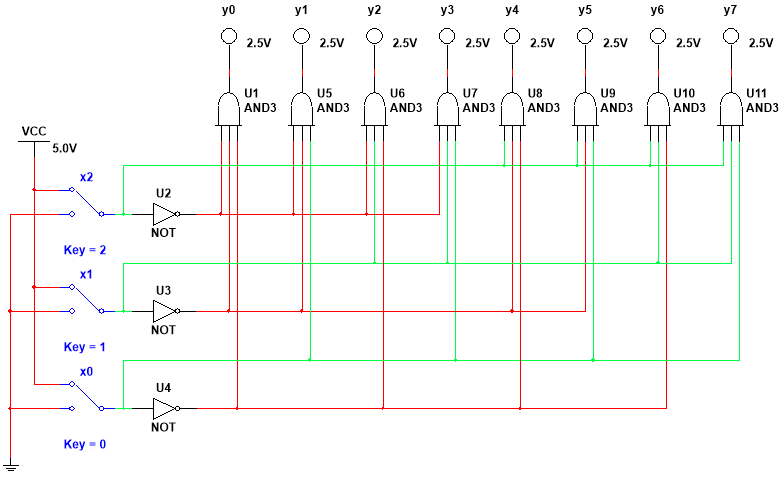
\includegraphics[width=0.85\textwidth]{painting_circuit.png}
	\caption{Схема электрическая принципиальная}
	\label{fig:painting_circuit}
\end{figure}

В следующей части лабораторной работы необходимо было изучить принцип работы дешифратора К155ИД4 (SN74155), схема которого приведена на на рис. \ref{fig:circuit_k155id4}. Была смоделирована схема в Multisim для проверки его работы, показанная на рис. \ref{fig:multisim_k155id4}.

\begin{figure}[H]
	\centering
	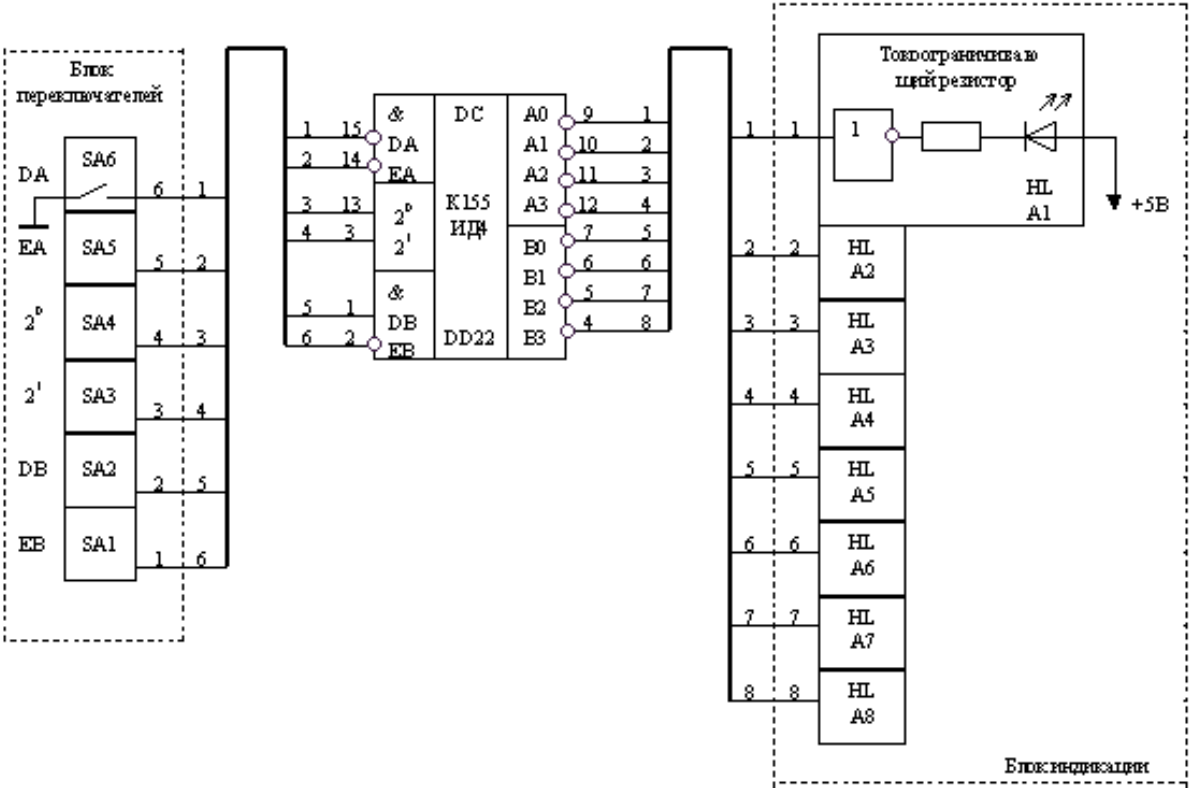
\includegraphics[width=0.85\textwidth]{circuit_k155id4.png}
	\caption{Схема дешифратора К155ИД4}
	\label{fig:circuit_k155id4}
\end{figure}

\begin{figure}[H]
	\centering
	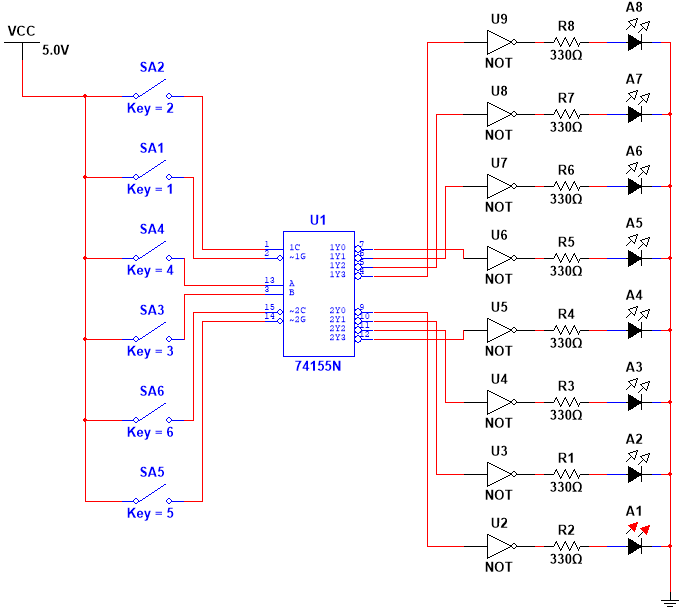
\includegraphics[width=0.85\textwidth]{multisim_k155id4.png}
	\caption{Схема дешифратора К155ИД4 в режиме 2х4 в Multisim}
	\label{fig:multisim_k155id4}
\end{figure}

Изменения схемы дешифратора для его работы в режиме 3 на 8 заключаются в объединении входов 1 и 15, 2 и 14. 

\begin{figure}[H]
	\centering
	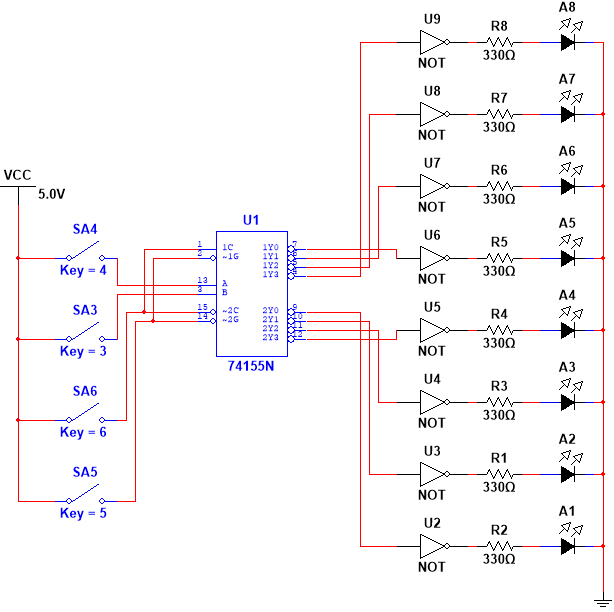
\includegraphics[width=0.85\textwidth]{multisim_k155id4_38.png}
	\caption{Схема дешифратора К155ИД4 в режиме 3х8 в Multisim}
	\label{fig:multisim_k155id4_38}
\end{figure}

\textbf{Выводы}

В ходе выполнения лабораторной работы были изучены теоретические основы построения и схемотехника комбинационных дешифраторов. На основе заданной таблицы истинности для каждого выхода $y_0 \dots y_7$ получены аналитические выражения в совершенной дизъюнктивной нормальной форме (СДНФ), по которым синтезирована и смоделирована принципиальная схема дешифратора 3х8 на логических элементах. Также исследована интегральная микросхема К155ИД4 (SN74155). Экспериментально проверено ее функционирование в режиме двух дешифраторов 2х4, а также подтверждена возможность объединения цепей для реализации полного дешифратора 3х8. Моделирование в среде Multisim полностью подтвердило соответствие работы исследуемых схем их теоретическим таблицам истинности.
%КАРТИНКИ
%\begin{figure}[H]
%	\centering
%	\includegraphics[width=0.85\textwidth]{install_deb.png}
%	\caption{Начало установки гостевой ОС Debian 12}
%	\label{fig:vbox_setup}
%\end{figure}

%---------------------------------------------------------------------------------
%ССЫЛКИ НА САЙТ

%\href{https://www.virtualbox.org/wiki/Downloads}{официального сайта VirtualBox}

%---------------------------------------------------------------------------------
%ССЫЛКА НА ПРИЛОЖЕНИЕ

%\texttt{zlib}\cite{zlib_docs}

%---------------------------------------------------------------------------------
%ССЫЛКА НА РИСУНОК

%показано на рис. \ref{fig:vbox_setup}

%---------------------------------------------------------------------------------
%ТАБЛИЦА С ПЕРЕВОДОМ НА СЛЕДУЮЩУЮ СТРАНИЦУ

%\begin{longtable}{|l|p{0.75\textwidth}|}
%	\caption{Функции библиотеки ncurses, используемые в TUI} \label{tab:ncurses_funcs} \\
%	\hline
%	\textbf{Функция} & \textbf{Назначение и описание алгоритма работы} \\ \hline
%	\endhead
%	\texttt{initscr()} & Инициализирует библиотеку, выделяет память под внутренние структуры окна и переводит терминал ОС в графический режим. \\ \hline
%	\texttt{cbreak()} & Отключает строковую буферизацию терминала, позволяя программе мгновенно реагировать на нажатия клавиш без ожидания \texttt{Enter}. \\ \hline
%	\texttt{noecho()} & Отключает автоматический вывод (эхо) вводимых пользователем символов на экран, позволяя программе самой управлять отрисовкой. \\ \hline
%	\texttt{clear()} & Очищает виртуальный экран для подготовки к отрисовке нового кадра меню. \\ \hline
%	\texttt{move(y, x)} & Осуществляет абсолютное позиционирование курсора по координатам \texttt{Y} (строка) и \texttt{X} (столбец). \\ \hline
%	\texttt{printw()} & Аналог функции \texttt{printf} для \texttt{ncurses}: выводит отформатированный текст в текущей позиции курсора. \\ \hline
%	\texttt{getch()} & Ожидает и считывает код нажатой пользователем клавиши (включая стрелки навигации и функциональные клавиши). \\ \hline
%	\texttt{getnstr()} & Безопасно считывает строку от пользователя с аппаратным ограничением максимального количества символов (защита от переполнения). \\ \hline
%	\texttt{scanw()} & Аналог функции \texttt{scanf}, считывает форматированный ввод пользователя (применяется для ввода числовых данных). \\ \hline
%	\texttt{endwin()} & Выгружает библиотеку из памяти, восстанавливает историю команд и возвращает терминал в стандартный режим работы ОС. \\ \hline
%\end{longtable}
%---------------------------------------------------------------------------------

\end{document}